% Options for packages loaded elsewhere
\PassOptionsToPackage{unicode}{hyperref}
\PassOptionsToPackage{hyphens}{url}
%
\documentclass[
]{article}
\usepackage{amsmath,amssymb}
\usepackage{iftex}
\ifPDFTeX
  \usepackage[T1]{fontenc}
  \usepackage[utf8]{inputenc}
  \usepackage{textcomp} % provide euro and other symbols
\else % if luatex or xetex
  \usepackage{unicode-math} % this also loads fontspec
  \defaultfontfeatures{Scale=MatchLowercase}
  \defaultfontfeatures[\rmfamily]{Ligatures=TeX,Scale=1}
\fi
\usepackage{lmodern}
\ifPDFTeX\else
  % xetex/luatex font selection
\fi
% Use upquote if available, for straight quotes in verbatim environments
\IfFileExists{upquote.sty}{\usepackage{upquote}}{}
\IfFileExists{microtype.sty}{% use microtype if available
  \usepackage[]{microtype}
  \UseMicrotypeSet[protrusion]{basicmath} % disable protrusion for tt fonts
}{}
\makeatletter
\@ifundefined{KOMAClassName}{% if non-KOMA class
  \IfFileExists{parskip.sty}{%
    \usepackage{parskip}
  }{% else
    \setlength{\parindent}{0pt}
    \setlength{\parskip}{6pt plus 2pt minus 1pt}}
}{% if KOMA class
  \KOMAoptions{parskip=half}}
\makeatother
\usepackage{xcolor}
\usepackage[margin=1in]{geometry}
\usepackage{color}
\usepackage{fancyvrb}
\newcommand{\VerbBar}{|}
\newcommand{\VERB}{\Verb[commandchars=\\\{\}]}
\DefineVerbatimEnvironment{Highlighting}{Verbatim}{commandchars=\\\{\}}
% Add ',fontsize=\small' for more characters per line
\usepackage{framed}
\definecolor{shadecolor}{RGB}{248,248,248}
\newenvironment{Shaded}{\begin{snugshade}}{\end{snugshade}}
\newcommand{\AlertTok}[1]{\textcolor[rgb]{0.94,0.16,0.16}{#1}}
\newcommand{\AnnotationTok}[1]{\textcolor[rgb]{0.56,0.35,0.01}{\textbf{\textit{#1}}}}
\newcommand{\AttributeTok}[1]{\textcolor[rgb]{0.13,0.29,0.53}{#1}}
\newcommand{\BaseNTok}[1]{\textcolor[rgb]{0.00,0.00,0.81}{#1}}
\newcommand{\BuiltInTok}[1]{#1}
\newcommand{\CharTok}[1]{\textcolor[rgb]{0.31,0.60,0.02}{#1}}
\newcommand{\CommentTok}[1]{\textcolor[rgb]{0.56,0.35,0.01}{\textit{#1}}}
\newcommand{\CommentVarTok}[1]{\textcolor[rgb]{0.56,0.35,0.01}{\textbf{\textit{#1}}}}
\newcommand{\ConstantTok}[1]{\textcolor[rgb]{0.56,0.35,0.01}{#1}}
\newcommand{\ControlFlowTok}[1]{\textcolor[rgb]{0.13,0.29,0.53}{\textbf{#1}}}
\newcommand{\DataTypeTok}[1]{\textcolor[rgb]{0.13,0.29,0.53}{#1}}
\newcommand{\DecValTok}[1]{\textcolor[rgb]{0.00,0.00,0.81}{#1}}
\newcommand{\DocumentationTok}[1]{\textcolor[rgb]{0.56,0.35,0.01}{\textbf{\textit{#1}}}}
\newcommand{\ErrorTok}[1]{\textcolor[rgb]{0.64,0.00,0.00}{\textbf{#1}}}
\newcommand{\ExtensionTok}[1]{#1}
\newcommand{\FloatTok}[1]{\textcolor[rgb]{0.00,0.00,0.81}{#1}}
\newcommand{\FunctionTok}[1]{\textcolor[rgb]{0.13,0.29,0.53}{\textbf{#1}}}
\newcommand{\ImportTok}[1]{#1}
\newcommand{\InformationTok}[1]{\textcolor[rgb]{0.56,0.35,0.01}{\textbf{\textit{#1}}}}
\newcommand{\KeywordTok}[1]{\textcolor[rgb]{0.13,0.29,0.53}{\textbf{#1}}}
\newcommand{\NormalTok}[1]{#1}
\newcommand{\OperatorTok}[1]{\textcolor[rgb]{0.81,0.36,0.00}{\textbf{#1}}}
\newcommand{\OtherTok}[1]{\textcolor[rgb]{0.56,0.35,0.01}{#1}}
\newcommand{\PreprocessorTok}[1]{\textcolor[rgb]{0.56,0.35,0.01}{\textit{#1}}}
\newcommand{\RegionMarkerTok}[1]{#1}
\newcommand{\SpecialCharTok}[1]{\textcolor[rgb]{0.81,0.36,0.00}{\textbf{#1}}}
\newcommand{\SpecialStringTok}[1]{\textcolor[rgb]{0.31,0.60,0.02}{#1}}
\newcommand{\StringTok}[1]{\textcolor[rgb]{0.31,0.60,0.02}{#1}}
\newcommand{\VariableTok}[1]{\textcolor[rgb]{0.00,0.00,0.00}{#1}}
\newcommand{\VerbatimStringTok}[1]{\textcolor[rgb]{0.31,0.60,0.02}{#1}}
\newcommand{\WarningTok}[1]{\textcolor[rgb]{0.56,0.35,0.01}{\textbf{\textit{#1}}}}
\usepackage{graphicx}
\makeatletter
\def\maxwidth{\ifdim\Gin@nat@width>\linewidth\linewidth\else\Gin@nat@width\fi}
\def\maxheight{\ifdim\Gin@nat@height>\textheight\textheight\else\Gin@nat@height\fi}
\makeatother
% Scale images if necessary, so that they will not overflow the page
% margins by default, and it is still possible to overwrite the defaults
% using explicit options in \includegraphics[width, height, ...]{}
\setkeys{Gin}{width=\maxwidth,height=\maxheight,keepaspectratio}
% Set default figure placement to htbp
\makeatletter
\def\fps@figure{htbp}
\makeatother
\setlength{\emergencystretch}{3em} % prevent overfull lines
\providecommand{\tightlist}{%
  \setlength{\itemsep}{0pt}\setlength{\parskip}{0pt}}
\setcounter{secnumdepth}{-\maxdimen} % remove section numbering
\ifLuaTeX
  \usepackage{selnolig}  % disable illegal ligatures
\fi
\IfFileExists{bookmark.sty}{\usepackage{bookmark}}{\usepackage{hyperref}}
\IfFileExists{xurl.sty}{\usepackage{xurl}}{} % add URL line breaks if available
\urlstyle{same}
\hypersetup{
  pdftitle={Supporting Information for},
  pdfauthor={James Boyko, Thais Vasconcelos},
  hidelinks,
  pdfcreator={LaTeX via pandoc}}

\title{Supporting Information for}
\usepackage{etoolbox}
\makeatletter
\providecommand{\subtitle}[1]{% add subtitle to \maketitle
  \apptocmd{\@title}{\par {\large #1 \par}}{}{}
}
\makeatother
\subtitle{Rates of biome shift predict diversification dynamics in
flowering plants.}
\author{James Boyko, Thais Vasconcelos}
\date{}

\begin{document}
\maketitle

\hypertarget{label-switching-and-the-impact-on-regression-results}{%
\subsection{Label switching and the impact on regression
results}\label{label-switching-and-the-impact-on-regression-results}}

One of the quirks of hidden Markov models (HMMs) is that the labeling of
rate classes is arbitrary. Not in the sense that labels are meaningless,
but rate that it makes no difference whether something is labeled as A
or B (a rate by any other name would smell as sweet).

This presents a problem for optimization since this means that there are
two parameterizations with exactly the same likelihood (swapping rate
class A and rate class B). Within packages like corHMM or hisse we have
tried to circumvent this issue by generally forcing one rate class to be
faster than another. This is done internally to help with the likelihood
search but should also provide more consistency in the output results.
Nonetheless, this issue could still impact our analysis of parameter
estimates.

The impact on our regression estimates would be due to the fact that
whether we are subtracting B from A is not consistent across our
datasets. This means that you could comfortably flip, for any given
clade, whether you are subtracting A from B or B from A. In this
vignette, I will run a randomization test to determine whether the
default results are trustworthy

Let's review our initial results.

\begin{verbatim}
## 
## Call:
## phylolm(formula = d_turns ~ d_trans, data = lm_dat, phy = phy_bb, 
##     boot = 1000)
## 
##    AIC logLik 
## 197.12 -95.56 
## 
## Raw residuals:
##     Min      1Q  Median      3Q     Max 
## -5.1012  0.2260  0.7647  1.2625  6.4253 
## 
## Mean tip height: 135.9122
## Parameter estimate(s) using ML:
## sigma2: 0.0296571 
## 
## Coefficients:
##              Estimate    StdErr   t.value lowerbootCI upperbootCI p.value  
## (Intercept) -0.695293  0.609029 -1.141642   -1.933491      0.4400 0.25939  
## d_trans      0.330045  0.135031  2.444214    0.046777      0.5907 0.01832 *
## ---
## Signif. codes:  0 '***' 0.001 '**' 0.01 '*' 0.05 '.' 0.1 ' ' 1
## 
## R-squared: 0.1128    Adjusted R-squared: 0.0939 
## 
## sigma2: 0.0296571
##       bootstrap mean: 0.02822535 (on raw scale)
##                       0.02765695 (on log scale, then back transformed)
##       bootstrap 95% CI: (0.01827899,0.04017403)
## 
## Parametric bootstrap results based on 1000 fitted replicates
\end{verbatim}

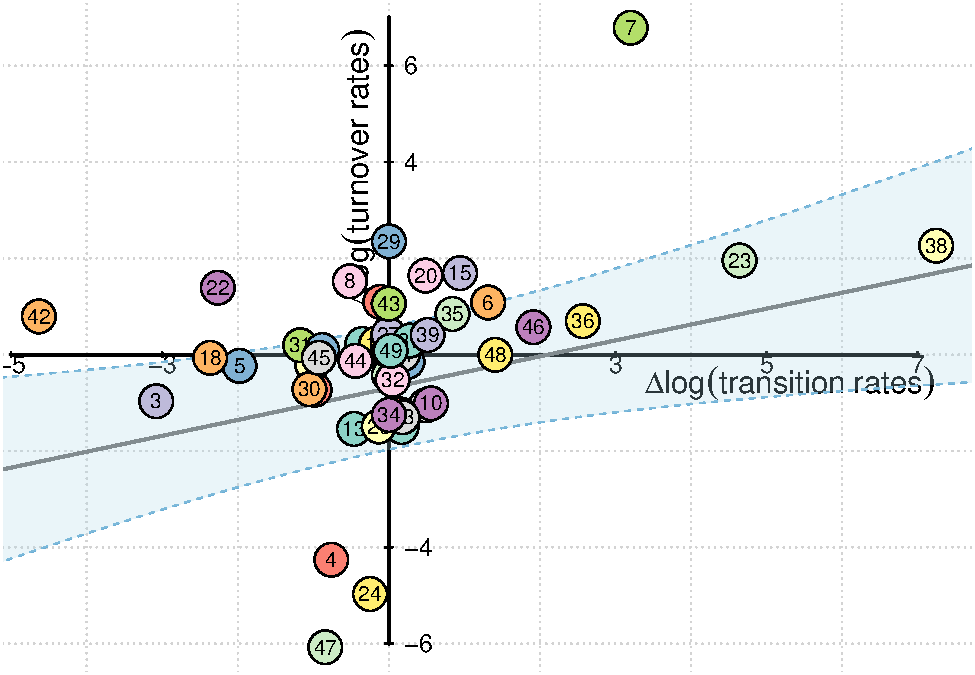
\includegraphics{SX-regression-distribution_files/figure-latex/unnamed-chunk-2-1.pdf}

The results of our initial regression are shown above. We find a
significant non-zero slope. However, as discussed above, for each clade,
rate class a and rate class b are interchangeable. If we shuffle the
rate classes around randomly, we will get a different result.

Let's look at the raw data as a starting point. The data shown below are
the transition rates for all possible transitions in our model with the
order as follows:
\(q_{00:01(A)},q_{01:00(A)},q_{01:11(A)},q_{11:01(A)},q_{00:01(B)},q_{01:00(B)},q_{01:11(B)},q_{11:01(B)}\)

\begin{Shaded}
\begin{Highlighting}[]
\NormalTok{demo\_df }\OtherTok{\textless{}{-}} \FunctionTok{data.frame}\NormalTok{( }\AttributeTok{a =} \FunctionTok{head}\NormalTok{(rate\_class\_a\_rate),}
                       \AttributeTok{b =} \FunctionTok{head}\NormalTok{(rate\_class\_b\_rate))}
\FunctionTok{print}\NormalTok{(demo\_df)}
\end{Highlighting}
\end{Shaded}

\begin{verbatim}
##          a.1         a.2        a.3        a.4        b.1       b.2        b.3
## 1  1.3326693  0.91372757  0.2759942  0.1598574 0.82861701 0.5864088  0.2800526
## 2  4.9219393  5.42387691 79.7965024 34.8578563 4.85165113 5.0091649 79.5819495
## 3  7.3769518 74.20552435 13.9641454 74.4910010 0.02403847 0.2138439  1.1785288
## 4  1.3308422 12.88786020  0.4080388  9.9758091 0.42336915 3.9711361  0.4093351
## 5 15.6736533  8.11807005 19.6690682  2.6754370 2.28548958 2.4752178  1.3565549
## 6  0.1514647  0.09133707  0.3293246  0.1734857 1.24066757 0.9679194  0.4678052
##           b.4
## 1  0.18960221
## 2 34.95402507
## 3  6.40132668
## 4  6.66990903
## 5  0.26680956
## 6  0.09777796
\end{verbatim}

\hypertarget{random-shuffling-for-a-null-distribution}{%
\subsection{Random shuffling for a null
distribution}\label{random-shuffling-for-a-null-distribution}}

To begin with let's try and examine a null expectation. In this case, if
we were to randomly shuffle all transition rates and turnover rates
(mixing rate class A and B) we would not expect to find an association.
By shuffling rate classes any estimated differences between rate class A
and rate class B should be removed.

\begin{Shaded}
\begin{Highlighting}[]
\NormalTok{shuffled\_rates }\OtherTok{\textless{}{-}} \FunctionTok{cbind}\NormalTok{(rate\_class\_a\_rate, rate\_class\_b\_rate)}
\NormalTok{shuffled\_rates }\OtherTok{\textless{}{-}} \FunctionTok{apply}\NormalTok{(shuffled\_rates, }\DecValTok{1}\NormalTok{, }
                        \ControlFlowTok{function}\NormalTok{(x) x[}\FunctionTok{sample}\NormalTok{(}\DecValTok{1}\SpecialCharTok{:}\DecValTok{8}\NormalTok{,}\DecValTok{8}\NormalTok{)])}
\NormalTok{shuffled\_rate\_class\_a\_rate }\OtherTok{\textless{}{-}} \FunctionTok{t}\NormalTok{(shuffled\_rates)[,}\DecValTok{1}\SpecialCharTok{:}\DecValTok{4}\NormalTok{]}
\NormalTok{shuffled\_rate\_class\_b\_rate }\OtherTok{\textless{}{-}} \FunctionTok{t}\NormalTok{(shuffled\_rates)[,}\DecValTok{5}\SpecialCharTok{:}\DecValTok{8}\NormalTok{]}


\NormalTok{shuffled\_turns }\OtherTok{\textless{}{-}} \FunctionTok{cbind}\NormalTok{(rate\_class\_a\_turn, rate\_class\_b\_turn)}
\NormalTok{shuffled\_turns }\OtherTok{\textless{}{-}} \FunctionTok{apply}\NormalTok{(shuffled\_turns, }\DecValTok{1}\NormalTok{, }
                        \ControlFlowTok{function}\NormalTok{(x) x[}\FunctionTok{sample}\NormalTok{(}\DecValTok{1}\SpecialCharTok{:}\DecValTok{6}\NormalTok{,}\DecValTok{6}\NormalTok{)])}
\NormalTok{shuffled\_rate\_class\_a\_turn }\OtherTok{\textless{}{-}} \FunctionTok{t}\NormalTok{(shuffled\_turns)[,}\DecValTok{1}\SpecialCharTok{:}\DecValTok{3}\NormalTok{]}
\NormalTok{shuffled\_rate\_class\_b\_turn }\OtherTok{\textless{}{-}} \FunctionTok{t}\NormalTok{(shuffled\_turns)[,}\DecValTok{4}\SpecialCharTok{:}\DecValTok{6}\NormalTok{]}

\NormalTok{d\_turns }\OtherTok{\textless{}{-}}\NormalTok{ d\_trans }\OtherTok{\textless{}{-}} \FunctionTok{c}\NormalTok{()}
\ControlFlowTok{for}\NormalTok{(i }\ControlFlowTok{in} \DecValTok{1}\SpecialCharTok{:}\DecValTok{49}\NormalTok{)\{}
\NormalTok{  d\_trans }\OtherTok{\textless{}{-}}\NormalTok{ (}\FunctionTok{c}\NormalTok{(d\_trans, }\FunctionTok{log}\NormalTok{(}\FunctionTok{rowMeans}\NormalTok{(shuffled\_rate\_class\_b\_rate)[i]) }\SpecialCharTok{{-}} 
                  \FunctionTok{log}\NormalTok{(}\FunctionTok{rowMeans}\NormalTok{(shuffled\_rate\_class\_a\_rate)[i])))}
\NormalTok{  d\_turns }\OtherTok{\textless{}{-}}\NormalTok{ (}\FunctionTok{c}\NormalTok{(d\_turns, }\FunctionTok{log}\NormalTok{(}\FunctionTok{rowMeans}\NormalTok{(shuffled\_rate\_class\_b\_turn)[i]) }\SpecialCharTok{{-}} 
                  \FunctionTok{log}\NormalTok{(}\FunctionTok{rowMeans}\NormalTok{(shuffled\_rate\_class\_a\_turn)[i])))}
\NormalTok{\}}

\NormalTok{lm\_dat\_null }\OtherTok{\textless{}{-}} \FunctionTok{data.frame}\NormalTok{(}\AttributeTok{row.names =} \FunctionTok{gsub}\NormalTok{(}\StringTok{" .*"}\NormalTok{, }\StringTok{""}\NormalTok{, plot\_data[,}\DecValTok{1}\NormalTok{]),}
                     \AttributeTok{d\_trans =}\NormalTok{ d\_trans,}
                     \AttributeTok{d\_turns =}\NormalTok{ d\_turns)}
\NormalTok{fit\_null }\OtherTok{=} \FunctionTok{phylolm}\NormalTok{(d\_turns }\SpecialCharTok{\textasciitilde{}}\NormalTok{ d\_trans, }\AttributeTok{data=}\NormalTok{lm\_dat\_null, }\AttributeTok{phy=}\NormalTok{phy\_bb, }\AttributeTok{boot =} \DecValTok{0}\NormalTok{)}
\FunctionTok{plot}\NormalTok{(lm\_dat\_null)}
\end{Highlighting}
\end{Shaded}

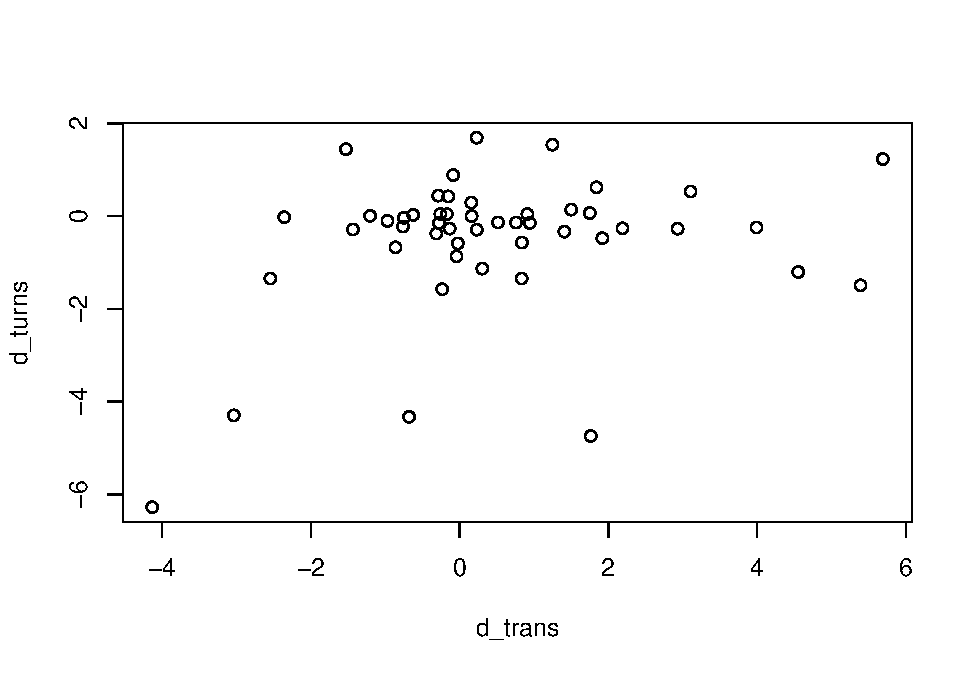
\includegraphics{SX-regression-distribution_files/figure-latex/unnamed-chunk-4-1.pdf}

\begin{Shaded}
\begin{Highlighting}[]
\FunctionTok{summary}\NormalTok{(fit\_null)}
\end{Highlighting}
\end{Shaded}

\begin{verbatim}
## 
## Call:
## phylolm(formula = d_turns ~ d_trans, data = lm_dat_null, phy = phy_bb, 
##     boot = 0)
## 
##    AIC logLik 
## 181.74 -87.87 
## 
## Raw residuals:
##     Min      1Q  Median      3Q     Max 
## -5.3965  0.3442  0.7772  0.9325  4.8922 
## 
## Mean tip height: 135.9122
## Parameter estimate(s) using ML:
## sigma2: 0.02167023 
## 
## Coefficients:
##             Estimate   StdErr t.value p.value
## (Intercept) -0.76505  0.52045  -1.470  0.1482
## d_trans      0.15119  0.13475   1.122  0.2676
## 
## R-squared: 0.02608   Adjusted R-squared: 0.005363
\end{verbatim}

This suggests this shuffling procedure did succesfully remove the signal
as the slope is not significantly different from 0. the Let's iterate
this shuffling procedure 1000 times and create a null distribution of
slope estimates.

\begin{Shaded}
\begin{Highlighting}[]
\NormalTok{all\_fits\_shuffled }\OtherTok{\textless{}{-}} \FunctionTok{list}\NormalTok{()}
\ControlFlowTok{for}\NormalTok{(j }\ControlFlowTok{in} \DecValTok{1}\SpecialCharTok{:}\DecValTok{1000}\NormalTok{)\{}
\NormalTok{  shuffled\_rates }\OtherTok{\textless{}{-}} \FunctionTok{cbind}\NormalTok{(rate\_class\_a\_rate, rate\_class\_b\_rate)}
\NormalTok{  shuffled\_rates }\OtherTok{\textless{}{-}} \FunctionTok{apply}\NormalTok{(shuffled\_rates, }\DecValTok{1}\NormalTok{, }
                          \ControlFlowTok{function}\NormalTok{(x) x[}\FunctionTok{sample}\NormalTok{(}\DecValTok{1}\SpecialCharTok{:}\DecValTok{8}\NormalTok{,}\DecValTok{8}\NormalTok{)])}
\NormalTok{  shuffled\_rate\_class\_a\_rate }\OtherTok{\textless{}{-}} \FunctionTok{t}\NormalTok{(shuffled\_rates)[,}\DecValTok{1}\SpecialCharTok{:}\DecValTok{4}\NormalTok{]}
\NormalTok{  shuffled\_rate\_class\_b\_rate }\OtherTok{\textless{}{-}} \FunctionTok{t}\NormalTok{(shuffled\_rates)[,}\DecValTok{5}\SpecialCharTok{:}\DecValTok{8}\NormalTok{]}
  
  
\NormalTok{  shuffled\_turns }\OtherTok{\textless{}{-}} \FunctionTok{cbind}\NormalTok{(rate\_class\_a\_turn, rate\_class\_b\_turn)}
\NormalTok{  shuffled\_turns }\OtherTok{\textless{}{-}} \FunctionTok{apply}\NormalTok{(shuffled\_turns, }\DecValTok{1}\NormalTok{, }
                          \ControlFlowTok{function}\NormalTok{(x) x[}\FunctionTok{sample}\NormalTok{(}\DecValTok{1}\SpecialCharTok{:}\DecValTok{6}\NormalTok{,}\DecValTok{6}\NormalTok{)])}
\NormalTok{  shuffled\_rate\_class\_a\_turn }\OtherTok{\textless{}{-}} \FunctionTok{t}\NormalTok{(shuffled\_turns)[,}\DecValTok{1}\SpecialCharTok{:}\DecValTok{3}\NormalTok{]}
\NormalTok{  shuffled\_rate\_class\_b\_turn }\OtherTok{\textless{}{-}} \FunctionTok{t}\NormalTok{(shuffled\_turns)[,}\DecValTok{4}\SpecialCharTok{:}\DecValTok{6}\NormalTok{]}
  
\NormalTok{  d\_turns }\OtherTok{\textless{}{-}}\NormalTok{ d\_trans }\OtherTok{\textless{}{-}} \FunctionTok{c}\NormalTok{()}
    \ControlFlowTok{for}\NormalTok{(i }\ControlFlowTok{in} \DecValTok{1}\SpecialCharTok{:}\DecValTok{49}\NormalTok{)\{}
\NormalTok{      d\_trans }\OtherTok{\textless{}{-}}\NormalTok{ (}\FunctionTok{c}\NormalTok{(d\_trans, }\FunctionTok{log}\NormalTok{(}\FunctionTok{rowMeans}\NormalTok{(shuffled\_rate\_class\_b\_rate)[i]) }\SpecialCharTok{{-}} 
                      \FunctionTok{log}\NormalTok{(}\FunctionTok{rowMeans}\NormalTok{(shuffled\_rate\_class\_a\_rate)[i])))}
\NormalTok{      d\_turns }\OtherTok{\textless{}{-}}\NormalTok{ (}\FunctionTok{c}\NormalTok{(d\_turns, }\FunctionTok{log}\NormalTok{(}\FunctionTok{rowMeans}\NormalTok{(shuffled\_rate\_class\_b\_turn)[i]) }\SpecialCharTok{{-}} 
                      \FunctionTok{log}\NormalTok{(}\FunctionTok{rowMeans}\NormalTok{(shuffled\_rate\_class\_a\_turn)[i])))}
\NormalTok{    \}}
\NormalTok{  lm\_dat\_shuffle }\OtherTok{\textless{}{-}} \FunctionTok{data.frame}\NormalTok{(}\AttributeTok{row.names =} \FunctionTok{gsub}\NormalTok{(}\StringTok{" .*"}\NormalTok{, }\StringTok{""}\NormalTok{, plot\_data[,}\DecValTok{1}\NormalTok{]),}
                       \AttributeTok{d\_trans =}\NormalTok{ d\_trans,}
                       \AttributeTok{d\_turns =}\NormalTok{ d\_turns)}
\NormalTok{  fit\_shuffle }\OtherTok{=} \FunctionTok{phylolm}\NormalTok{(d\_turns }\SpecialCharTok{\textasciitilde{}}\NormalTok{ d\_trans, }\AttributeTok{data=}\NormalTok{lm\_dat\_shuffle, }\AttributeTok{phy=}\NormalTok{phy\_bb, }\AttributeTok{boot =} \DecValTok{0}\NormalTok{)}
\NormalTok{  all\_fits\_shuffled[[j]] }\OtherTok{\textless{}{-}}\NormalTok{ fit\_shuffle}
\NormalTok{\}}
\end{Highlighting}
\end{Shaded}

Distribution of the p-values and slope estimates.

\begin{Shaded}
\begin{Highlighting}[]
\NormalTok{shuffled\_est }\OtherTok{\textless{}{-}} \FunctionTok{lapply}\NormalTok{(all\_fits\_shuffled, }
                       \ControlFlowTok{function}\NormalTok{(x) }\FunctionTok{summary}\NormalTok{(x)}\SpecialCharTok{$}\NormalTok{coefficients[}\DecValTok{2}\NormalTok{,}\FunctionTok{c}\NormalTok{(}\DecValTok{1}\NormalTok{,}\DecValTok{4}\NormalTok{)])}
\NormalTok{shuffled\_est\_df }\OtherTok{\textless{}{-}} \FunctionTok{do.call}\NormalTok{(rbind,shuffled\_est)}

\FunctionTok{par}\NormalTok{(}\AttributeTok{mfrow=}\FunctionTok{c}\NormalTok{(}\DecValTok{1}\NormalTok{,}\DecValTok{2}\NormalTok{))}
\FunctionTok{hist}\NormalTok{(shuffled\_est\_df[,}\DecValTok{1}\NormalTok{], }\AttributeTok{main =} \StringTok{"slope estimates"}\NormalTok{, }\AttributeTok{xlab =} \StringTok{"slope value"}\NormalTok{)}
\FunctionTok{hist}\NormalTok{(shuffled\_est\_df[,}\DecValTok{2}\NormalTok{], }\AttributeTok{main =} \StringTok{"p{-}values"}\NormalTok{, }\AttributeTok{xlab =} \StringTok{"pvalue"}\NormalTok{)}
\end{Highlighting}
\end{Shaded}

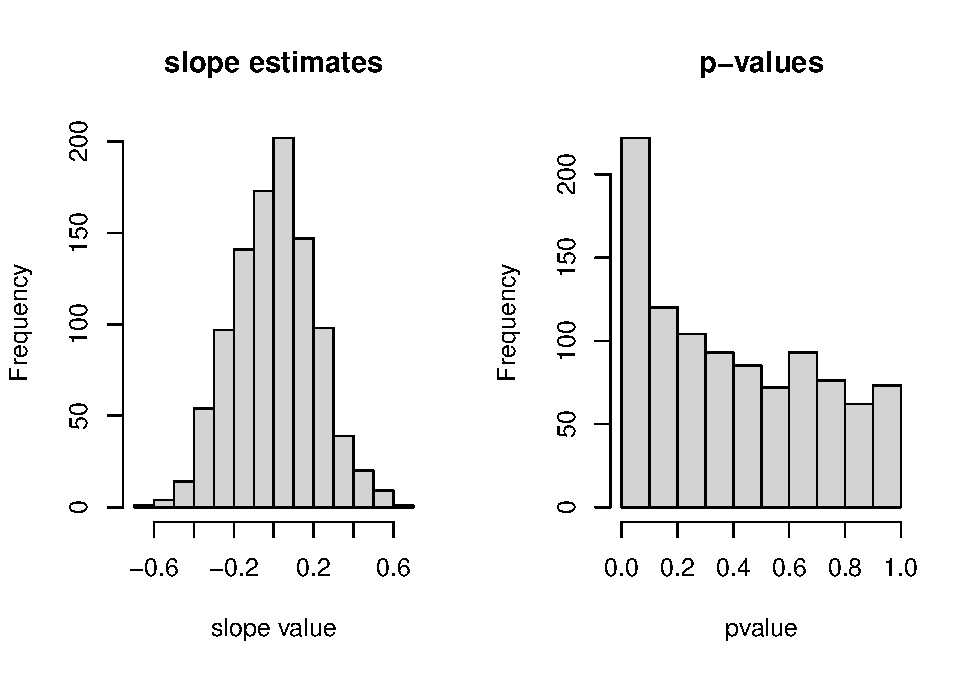
\includegraphics{SX-regression-distribution_files/figure-latex/unnamed-chunk-7-1.pdf}

\hypertarget{random-shuffling-for-robustness-against-label-switching}{%
\subsection{Random shuffling for robustness against label
switching}\label{random-shuffling-for-robustness-against-label-switching}}

With a null expectation established let's shuffle rate classes in a way
that should preserve the signal by randomly shuffling labels. The
shuffling will randomly select between 1 and 49 clades and then randomly
choose which of those clades will swap the labels on the rate class A
and B.

\begin{Shaded}
\begin{Highlighting}[]
\NormalTok{no\_to\_swap }\OtherTok{\textless{}{-}} \FunctionTok{sample}\NormalTok{(}\DecValTok{1}\SpecialCharTok{:}\DecValTok{49}\NormalTok{, }\DecValTok{1}\NormalTok{)}
\NormalTok{to\_swap }\OtherTok{\textless{}{-}} \FunctionTok{sample}\NormalTok{(}\DecValTok{1}\SpecialCharTok{:}\DecValTok{49}\NormalTok{, no\_to\_swap, }\ConstantTok{FALSE}\NormalTok{)}
\NormalTok{d\_turns }\OtherTok{\textless{}{-}}\NormalTok{ d\_trans }\OtherTok{\textless{}{-}} \FunctionTok{c}\NormalTok{()}
\ControlFlowTok{for}\NormalTok{(i }\ControlFlowTok{in} \DecValTok{1}\SpecialCharTok{:}\DecValTok{49}\NormalTok{)\{}
  \ControlFlowTok{if}\NormalTok{(i }\SpecialCharTok{\%in\%}\NormalTok{ to\_swap)\{}
\NormalTok{    d\_trans }\OtherTok{\textless{}{-}}\NormalTok{ (}\FunctionTok{c}\NormalTok{(d\_trans, }\FunctionTok{log}\NormalTok{(}\FunctionTok{rowMeans}\NormalTok{(rate\_class\_a\_rate)[i]) }\SpecialCharTok{{-}} 
                    \FunctionTok{log}\NormalTok{(}\FunctionTok{rowMeans}\NormalTok{(rate\_class\_b\_rate)[i])))}
\NormalTok{    d\_turns }\OtherTok{\textless{}{-}}\NormalTok{ (}\FunctionTok{c}\NormalTok{(d\_turns, }\FunctionTok{log}\NormalTok{(}\FunctionTok{rowMeans}\NormalTok{(rate\_class\_a\_turn)[i]) }\SpecialCharTok{{-}} 
                    \FunctionTok{log}\NormalTok{(}\FunctionTok{rowMeans}\NormalTok{(rate\_class\_b\_turn)[i])))}
\NormalTok{  \}}\ControlFlowTok{else}\NormalTok{\{}
\NormalTok{    d\_trans }\OtherTok{\textless{}{-}}\NormalTok{ (}\FunctionTok{c}\NormalTok{(d\_trans, }\FunctionTok{log}\NormalTok{(}\FunctionTok{rowMeans}\NormalTok{(rate\_class\_b\_rate)[i]) }\SpecialCharTok{{-}} 
                    \FunctionTok{log}\NormalTok{(}\FunctionTok{rowMeans}\NormalTok{(rate\_class\_a\_rate)[i])))}
\NormalTok{    d\_turns }\OtherTok{\textless{}{-}}\NormalTok{ (}\FunctionTok{c}\NormalTok{(d\_turns, }\FunctionTok{log}\NormalTok{(}\FunctionTok{rowMeans}\NormalTok{(rate\_class\_b\_turn)[i]) }\SpecialCharTok{{-}} 
                    \FunctionTok{log}\NormalTok{(}\FunctionTok{rowMeans}\NormalTok{(rate\_class\_a\_turn)[i])))}
\NormalTok{  \}}
\NormalTok{\}}

\NormalTok{lm\_dat\_shuffle }\OtherTok{\textless{}{-}} \FunctionTok{data.frame}\NormalTok{(}\AttributeTok{row.names =} \FunctionTok{gsub}\NormalTok{(}\StringTok{" .*"}\NormalTok{, }\StringTok{""}\NormalTok{, plot\_data[,}\DecValTok{1}\NormalTok{]),}
                     \AttributeTok{d\_trans =}\NormalTok{ d\_trans,}
                     \AttributeTok{d\_turns =}\NormalTok{ d\_turns)}
\NormalTok{fit\_shuffle }\OtherTok{=} \FunctionTok{phylolm}\NormalTok{(d\_turns }\SpecialCharTok{\textasciitilde{}}\NormalTok{ d\_trans, }\AttributeTok{data=}\NormalTok{lm\_dat\_shuffle, }\AttributeTok{phy=}\NormalTok{phy\_bb, }\AttributeTok{boot =} \DecValTok{0}\NormalTok{)}
\FunctionTok{plot}\NormalTok{(lm\_dat\_shuffle)}
\end{Highlighting}
\end{Shaded}

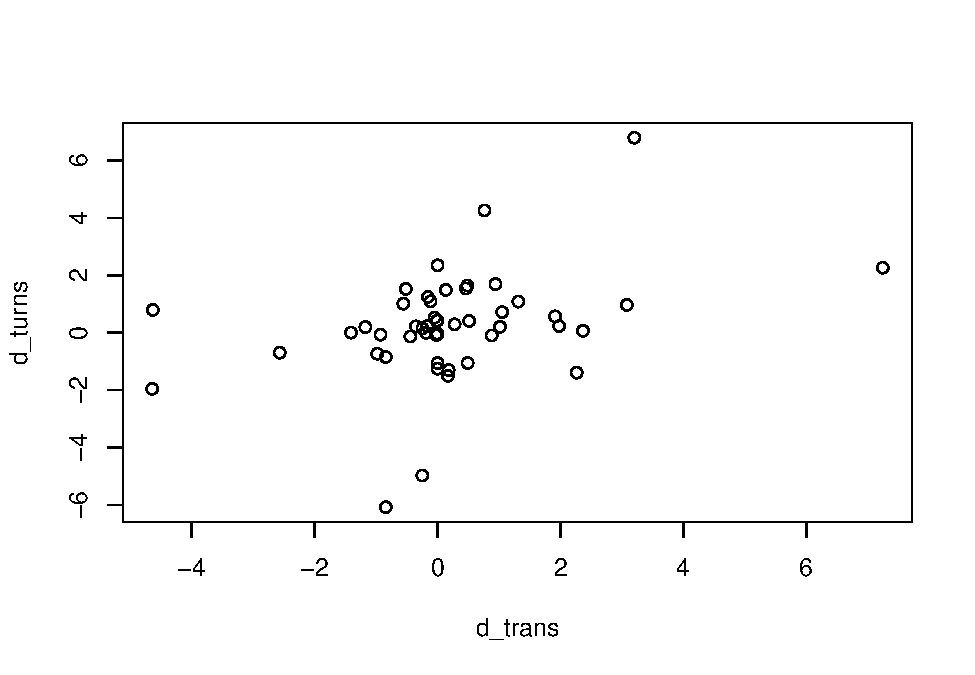
\includegraphics{SX-regression-distribution_files/figure-latex/unnamed-chunk-8-1.pdf}

If we look at the data we can see that the data has been shuffled.

\begin{Shaded}
\begin{Highlighting}[]
\FunctionTok{summary}\NormalTok{(fit\_shuffle)}
\end{Highlighting}
\end{Shaded}

\begin{verbatim}
## 
## Call:
## phylolm(formula = d_turns ~ d_trans, data = lm_dat_shuffle, phy = phy_bb, 
##     boot = 0)
## 
##    AIC logLik 
## 198.76 -96.38 
## 
## Raw residuals:
##     Min      1Q  Median      3Q     Max 
## -5.2443  0.1459  0.6333  1.2257  6.3273 
## 
## Mean tip height: 135.9122
## Parameter estimate(s) using ML:
## sigma2: 0.03066753 
## 
## Coefficients:
##             Estimate   StdErr t.value p.value  
## (Intercept) -0.56159  0.61963 -0.9063 0.36938  
## d_trans      0.31890  0.13548  2.3539 0.02281 *
## ---
## Signif. codes:  0 '***' 0.001 '**' 0.01 '*' 0.05 '.' 0.1 ' ' 1
## 
## R-squared: 0.1055    Adjusted R-squared: 0.08643
\end{verbatim}

However, we are still able to recover a significantly positive slope.
Lets repeat this procedure 1000 times.

\begin{Shaded}
\begin{Highlighting}[]
\NormalTok{all\_fits }\OtherTok{\textless{}{-}} \FunctionTok{list}\NormalTok{()}
\ControlFlowTok{for}\NormalTok{(j }\ControlFlowTok{in} \DecValTok{1}\SpecialCharTok{:}\DecValTok{1000}\NormalTok{)\{}
\NormalTok{  no\_to\_swap }\OtherTok{\textless{}{-}} \FunctionTok{sample}\NormalTok{(}\DecValTok{1}\SpecialCharTok{:}\DecValTok{49}\NormalTok{, }\DecValTok{1}\NormalTok{)}
\NormalTok{  to\_swap }\OtherTok{\textless{}{-}} \FunctionTok{sample}\NormalTok{(}\DecValTok{1}\SpecialCharTok{:}\DecValTok{49}\NormalTok{, no\_to\_swap, }\ConstantTok{FALSE}\NormalTok{)}
\NormalTok{  d\_turns }\OtherTok{\textless{}{-}}\NormalTok{ d\_trans }\OtherTok{\textless{}{-}} \FunctionTok{c}\NormalTok{()}
  \ControlFlowTok{for}\NormalTok{(i }\ControlFlowTok{in} \DecValTok{1}\SpecialCharTok{:}\DecValTok{49}\NormalTok{)\{}
    \ControlFlowTok{if}\NormalTok{(i }\SpecialCharTok{\%in\%}\NormalTok{ to\_swap)\{}
\NormalTok{      d\_trans }\OtherTok{\textless{}{-}}\NormalTok{ (}\FunctionTok{c}\NormalTok{(d\_trans, }\FunctionTok{log}\NormalTok{(}\FunctionTok{rowMeans}\NormalTok{(rate\_class\_a\_rate)[i]) }\SpecialCharTok{{-}} 
                      \FunctionTok{log}\NormalTok{(}\FunctionTok{rowMeans}\NormalTok{(rate\_class\_b\_rate)[i])))}
\NormalTok{      d\_turns }\OtherTok{\textless{}{-}}\NormalTok{ (}\FunctionTok{c}\NormalTok{(d\_turns, }\FunctionTok{log}\NormalTok{(}\FunctionTok{rowMeans}\NormalTok{(rate\_class\_a\_turn)[i]) }\SpecialCharTok{{-}} 
                      \FunctionTok{log}\NormalTok{(}\FunctionTok{rowMeans}\NormalTok{(rate\_class\_b\_turn)[i])))}
\NormalTok{    \}}\ControlFlowTok{else}\NormalTok{\{}
\NormalTok{      d\_trans }\OtherTok{\textless{}{-}}\NormalTok{ (}\FunctionTok{c}\NormalTok{(d\_trans, }\FunctionTok{log}\NormalTok{(}\FunctionTok{rowMeans}\NormalTok{(rate\_class\_b\_rate)[i]) }\SpecialCharTok{{-}} 
                      \FunctionTok{log}\NormalTok{(}\FunctionTok{rowMeans}\NormalTok{(rate\_class\_a\_rate)[i])))}
\NormalTok{      d\_turns }\OtherTok{\textless{}{-}}\NormalTok{ (}\FunctionTok{c}\NormalTok{(d\_turns, }\FunctionTok{log}\NormalTok{(}\FunctionTok{rowMeans}\NormalTok{(rate\_class\_b\_turn)[i]) }\SpecialCharTok{{-}} 
                      \FunctionTok{log}\NormalTok{(}\FunctionTok{rowMeans}\NormalTok{(rate\_class\_a\_turn)[i])))}
\NormalTok{    \}}
\NormalTok{  \}}
  
\NormalTok{  lm\_dat\_tmp }\OtherTok{\textless{}{-}} \FunctionTok{data.frame}\NormalTok{(}\AttributeTok{row.names =} \FunctionTok{gsub}\NormalTok{(}\StringTok{" .*"}\NormalTok{, }\StringTok{""}\NormalTok{, plot\_data[,}\DecValTok{1}\NormalTok{]),}
                       \AttributeTok{d\_trans =}\NormalTok{ d\_trans,}
                       \AttributeTok{d\_turns =}\NormalTok{ d\_turns)}
\NormalTok{  fit\_tmp }\OtherTok{=} \FunctionTok{phylolm}\NormalTok{(d\_turns }\SpecialCharTok{\textasciitilde{}}\NormalTok{ d\_trans, }\AttributeTok{data=}\NormalTok{lm\_dat\_tmp, }\AttributeTok{phy=}\NormalTok{phy\_bb, }\AttributeTok{boot =} \DecValTok{0}\NormalTok{)}
\NormalTok{  all\_fits[[j]] }\OtherTok{\textless{}{-}}\NormalTok{ fit\_tmp}
\NormalTok{\}}
\end{Highlighting}
\end{Shaded}

Let's plot the resulting distributions.

\begin{Shaded}
\begin{Highlighting}[]
\NormalTok{est }\OtherTok{\textless{}{-}} \FunctionTok{lapply}\NormalTok{(all\_fits, }
              \ControlFlowTok{function}\NormalTok{(x) }\FunctionTok{summary}\NormalTok{(x)}\SpecialCharTok{$}\NormalTok{coefficients[}\DecValTok{2}\NormalTok{,}\FunctionTok{c}\NormalTok{(}\DecValTok{1}\NormalTok{,}\DecValTok{4}\NormalTok{)])}
\NormalTok{est\_df }\OtherTok{\textless{}{-}} \FunctionTok{do.call}\NormalTok{(rbind,est)}

\FunctionTok{par}\NormalTok{(}\AttributeTok{mfrow=}\FunctionTok{c}\NormalTok{(}\DecValTok{1}\NormalTok{,}\DecValTok{2}\NormalTok{))}
\FunctionTok{hist}\NormalTok{(est\_df[,}\DecValTok{1}\NormalTok{], }\AttributeTok{main =} \StringTok{"slope estimates"}\NormalTok{, }\AttributeTok{xlab =} \StringTok{"slope value"}\NormalTok{)}
\FunctionTok{hist}\NormalTok{(est\_df[,}\DecValTok{2}\NormalTok{], }\AttributeTok{main =} \StringTok{"p{-}values"}\NormalTok{, }\AttributeTok{xlab =} \StringTok{"pvalue"}\NormalTok{)}
\end{Highlighting}
\end{Shaded}

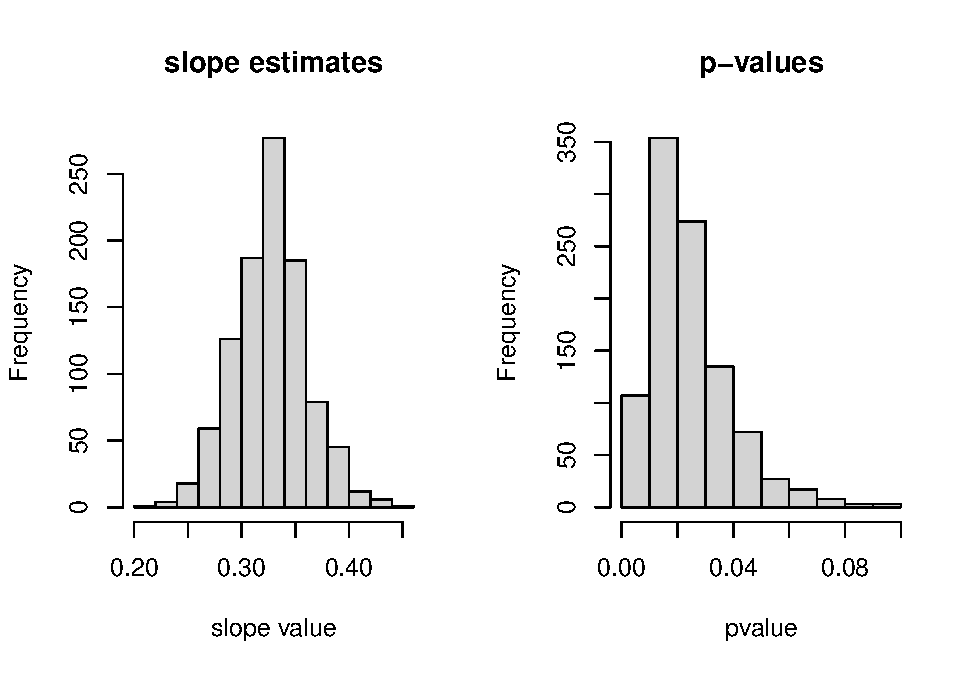
\includegraphics{SX-regression-distribution_files/figure-latex/unnamed-chunk-11-1.pdf}

\hypertarget{comparing-distributions}{%
\subsection{Comparing distributions}\label{comparing-distributions}}

\begin{Shaded}
\begin{Highlighting}[]
\CommentTok{\# Calculate the combined range for the slope estimates}
\NormalTok{min\_slope }\OtherTok{=} \FunctionTok{min}\NormalTok{(}\FunctionTok{c}\NormalTok{(shuffled\_est\_df[,}\DecValTok{1}\NormalTok{], est\_df[,}\DecValTok{1}\NormalTok{]))}
\NormalTok{max\_slope }\OtherTok{=} \FunctionTok{max}\NormalTok{(}\FunctionTok{c}\NormalTok{(shuffled\_est\_df[,}\DecValTok{1}\NormalTok{], est\_df[,}\DecValTok{1}\NormalTok{]))}

\CommentTok{\# Calculate the combined range for the p{-}values}
\NormalTok{min\_pvalue }\OtherTok{=} \FunctionTok{min}\NormalTok{(}\FunctionTok{c}\NormalTok{(shuffled\_est\_df[,}\DecValTok{2}\NormalTok{], est\_df[,}\DecValTok{2}\NormalTok{]))}
\NormalTok{max\_pvalue }\OtherTok{=} \FunctionTok{max}\NormalTok{(}\FunctionTok{c}\NormalTok{(shuffled\_est\_df[,}\DecValTok{2}\NormalTok{], est\_df[,}\DecValTok{2}\NormalTok{]))}

\CommentTok{\# Define uniform break points for both datasets}
\NormalTok{breaks\_slope }\OtherTok{=} \FunctionTok{seq}\NormalTok{(min\_slope, max\_slope, }\AttributeTok{length.out=}\DecValTok{31}\NormalTok{)  }\CommentTok{\# 30 bins, adjust number of breaks as needed}
\NormalTok{breaks\_pvalue }\OtherTok{=} \FunctionTok{seq}\NormalTok{(min\_pvalue, max\_pvalue, }\AttributeTok{length.out=}\DecValTok{31}\NormalTok{)  }\CommentTok{\# 30 bins}

\FunctionTok{par}\NormalTok{(}\AttributeTok{mfrow=}\FunctionTok{c}\NormalTok{(}\DecValTok{1}\NormalTok{,}\DecValTok{2}\NormalTok{))}
\CommentTok{\# Plot histograms for slope estimates}
\FunctionTok{hist}\NormalTok{(shuffled\_est\_df[,}\DecValTok{1}\NormalTok{], }\AttributeTok{breaks=}\NormalTok{breaks\_slope, }\AttributeTok{main=}\StringTok{"Overlay of Slope Estimates"}\NormalTok{, }\AttributeTok{xlab=}\StringTok{"Slope Value"}\NormalTok{, }\AttributeTok{col=}\FunctionTok{rgb}\NormalTok{(}\DecValTok{1}\NormalTok{, }\DecValTok{0}\NormalTok{, }\DecValTok{0}\NormalTok{, }\FloatTok{0.5}\NormalTok{), }\AttributeTok{ylim=}\FunctionTok{c}\NormalTok{(}\DecValTok{0}\NormalTok{, }\FunctionTok{max}\NormalTok{(}\FunctionTok{c}\NormalTok{(}\FunctionTok{hist}\NormalTok{(shuffled\_est\_df[,}\DecValTok{1}\NormalTok{], }\AttributeTok{breaks=}\NormalTok{breaks\_slope, }\AttributeTok{plot=}\ConstantTok{FALSE}\NormalTok{)}\SpecialCharTok{$}\NormalTok{counts, }\FunctionTok{hist}\NormalTok{(est\_df[,}\DecValTok{1}\NormalTok{], }\AttributeTok{breaks=}\NormalTok{breaks\_slope, }\AttributeTok{plot=}\ConstantTok{FALSE}\NormalTok{)}\SpecialCharTok{$}\NormalTok{counts))))}
\FunctionTok{hist}\NormalTok{(est\_df[,}\DecValTok{1}\NormalTok{], }\AttributeTok{breaks=}\NormalTok{breaks\_slope, }\AttributeTok{add=}\ConstantTok{TRUE}\NormalTok{, }\AttributeTok{col=}\FunctionTok{rgb}\NormalTok{(}\DecValTok{0}\NormalTok{, }\DecValTok{0}\NormalTok{, }\DecValTok{1}\NormalTok{, }\FloatTok{0.5}\NormalTok{))}
\FunctionTok{legend}\NormalTok{(}\StringTok{"topleft"}\NormalTok{, }\AttributeTok{legend=}\FunctionTok{c}\NormalTok{(}\StringTok{"Null"}\NormalTok{, }\StringTok{"Labels shuffled"}\NormalTok{), }\AttributeTok{fill=}\FunctionTok{c}\NormalTok{(}\FunctionTok{rgb}\NormalTok{(}\DecValTok{1}\NormalTok{, }\DecValTok{0}\NormalTok{, }\DecValTok{0}\NormalTok{, }\FloatTok{0.5}\NormalTok{), }\FunctionTok{rgb}\NormalTok{(}\DecValTok{0}\NormalTok{, }\DecValTok{0}\NormalTok{, }\DecValTok{1}\NormalTok{, }\FloatTok{0.5}\NormalTok{)),}\AttributeTok{bty =} \StringTok{"n"}\NormalTok{, }\AttributeTok{cex=}\FloatTok{0.75}\NormalTok{)}

\CommentTok{\# Plot histograms for p{-}values}
\FunctionTok{hist}\NormalTok{(shuffled\_est\_df[,}\DecValTok{2}\NormalTok{], }\AttributeTok{breaks=}\NormalTok{breaks\_pvalue, }\AttributeTok{main=}\StringTok{"Overlay of P{-}values"}\NormalTok{, }\AttributeTok{xlab=}\StringTok{"P{-}value"}\NormalTok{, }\AttributeTok{col=}\FunctionTok{rgb}\NormalTok{(}\DecValTok{1}\NormalTok{, }\DecValTok{0}\NormalTok{, }\DecValTok{0}\NormalTok{, }\FloatTok{0.5}\NormalTok{), }\AttributeTok{ylim=}\FunctionTok{c}\NormalTok{(}\DecValTok{0}\NormalTok{, }\FunctionTok{max}\NormalTok{(}\FunctionTok{c}\NormalTok{(}\FunctionTok{hist}\NormalTok{(shuffled\_est\_df[,}\DecValTok{2}\NormalTok{], }\AttributeTok{breaks=}\NormalTok{breaks\_pvalue, }\AttributeTok{plot=}\ConstantTok{FALSE}\NormalTok{)}\SpecialCharTok{$}\NormalTok{counts, }\FunctionTok{hist}\NormalTok{(est\_df[,}\DecValTok{2}\NormalTok{], }\AttributeTok{breaks=}\NormalTok{breaks\_pvalue, }\AttributeTok{plot=}\ConstantTok{FALSE}\NormalTok{)}\SpecialCharTok{$}\NormalTok{counts))))}
\FunctionTok{hist}\NormalTok{(est\_df[,}\DecValTok{2}\NormalTok{], }\AttributeTok{breaks=}\NormalTok{breaks\_pvalue, }\AttributeTok{add=}\ConstantTok{TRUE}\NormalTok{, }\AttributeTok{col=}\FunctionTok{rgb}\NormalTok{(}\DecValTok{0}\NormalTok{, }\DecValTok{0}\NormalTok{, }\DecValTok{1}\NormalTok{, }\FloatTok{0.5}\NormalTok{))}
\end{Highlighting}
\end{Shaded}

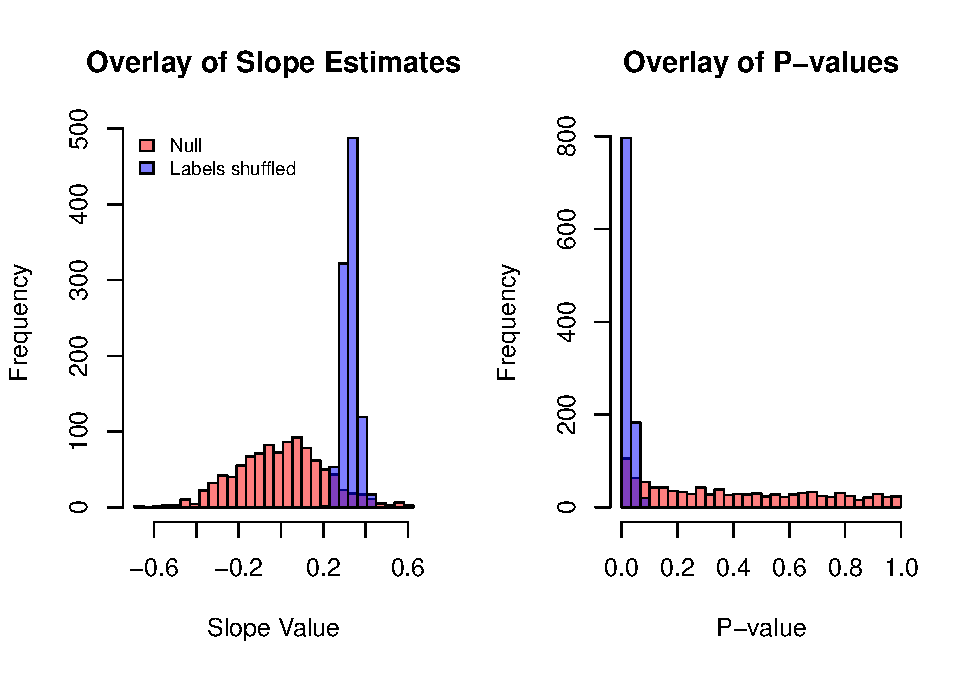
\includegraphics{SX-regression-distribution_files/figure-latex/unnamed-chunk-12-1.pdf}

This suggests that our results are robust to the label switching problem
with average estimates shown below.

\begin{verbatim}
## [1] "mean null"
\end{verbatim}

\begin{verbatim}
##    Estimate     p.value 
## -0.01729697  0.38927046
\end{verbatim}

\begin{verbatim}
## [1] "mean labels switched"
\end{verbatim}

\begin{verbatim}
##   Estimate    p.value 
## 0.32754067 0.02395771
\end{verbatim}

\end{document}
